\documentclass[11pt]{article}

\usepackage[letterpaper, margin=1in]{geometry}

\usepackage[spanish]{babel}
\usepackage[utf8]{inputenc}
\usepackage{multirow}
\usepackage{tabularx}
\usepackage{longtable}

%para poder poner codigo en colores
\usepackage[dvipsnames]{xcolor}
\definecolor{dkgreen}{rgb}{0,0.6,0}
\definecolor{gray}{rgb}{0.5,0.5,0.5}
\definecolor{mauve}{rgb}{0.58,0,0.82}

%Figuras
\usepackage{graphicx, subfigure}
\usepackage[]{tikz}
\usepackage{pbox}
%Matemática
\usepackage{amsmath}
\usepackage{amssymb}
%Símbolos mate extra (alfabetos, etc.)
\usepackage{mathrsfs}
%Algoritmos
\usepackage{float}
\usepackage{algorithm}
\usepackage{algorithmicx}
\usepackage{algpseudocode}
\usepackage{listings}

\usepackage{color}
\usepackage{hyperref}

\usepackage{mdframed}
\usepackage{tcolorbox}
\usepackage{multicol}
\usepackage{booktabs}
\usepackage{tabulary}
\definecolor{darkblue}{rgb}{0 , 0.054 , 0.196}

%para poder poner codigo en colores
\lstset{frame=tb,
  language=c++,
  aboveskip=3mm,
  belowskip=3mm,
  showstringspaces=false,
  columns=flexible,
  basicstyle={\small\ttfamily},
  numbers=none,
  numberstyle=\tiny\color{gray},
  keywordstyle=\color{blue},
  commentstyle=\color{dkgreen},
  stringstyle=\color{cyan},
  breaklines=true,
  breakatwhitespace=true,
  tabsize=3
}


\title{Reporte Laboratorio 2: \\ Estructuras de datos lineales}
\author{Luis Adrian Aguilar Casacante - B00092\\Robin González - B43011\\Giancarlo Marín - B54099}

\begin{document}

\maketitle
\hrule
\hrule
\tableofcontents
\hspace{5mm}
\hrule
\hrule

\hfill
\hfill
\newpage
\section{Enunciado}
Implementar las estructuras lineales de datos utilizando plantillas, herencia y POO en C++, siguiendo los lineamientos del archivo List.h. Las estructuras que debe implementar recibirán en los argumentos de la plantilla dos elementos: el tipo de dato que almacenará y el tipo que utilizará como posición (lo que determinará su implementación subyacente).\\
\begin{enumerate}
\item Lista con arreglos: en un archivo llamado ListWithArray.h Esta clase debe heredar de la clase List.
\item Lista con punteros: en un archivo llamado ListWithPointer.h. Esta clase debe heredar de la clase List. Para la posición implemente una clase emplantillada llamada Cell que reciba el dato que almacenará.
\item Cola: en un archivo llamado Queue.h y usando una plantilla que reciba el tipo de dato que usará la cola y el tipo de posición que utilizará. Esta clase debe heredar de la clase List. Es de notar que la cola es una lista con restricciones por lo que es posible que no todos los métodos de las listas tengan sentido.
\item Pila: en un archivo llamado Stack.h y usando una plantilla que reciba el tipo de dato que usará la cola y el tipo de posición que utilizará. Esta clase debe heredar de la clase List. Es de notar que la cola es una lista con restricciones por lo que es posible que no todos los métodos de las listas tengan sentido.
\item Haga un programa de prueba para sus estructuras. Asegúrese de hacer inserciones y borrados al inicio, al final y en medio de las listas. Por último realice una revisión de:
\begin{itemize}
\item Colas de prioridad
\item Coladoble
\end{itemize}
\end{enumerate}

\section{Introducción}
En el presente laboratorio, se realiza la implementación de distintas Estructuras de Datos Abstractas (ADT por sus siglas en inglés) de datos lineales como lo son las Listas, Pilas y Colas.

Una pila es una estructura de datos en la cual los elementos almacenados en la misma se agregan y se sacan del mismo lugar (LIFO), llamado el tope de la pila (top). Por su parte, una cola es una estructura de datos en la cual los elementos almacenados se agregan al final y se sacan del principio de la cola (LIFO). 
\\La otra estructura implementada es la lista, en esta se pueden agregar, borrar y acceder los elementos sin restricciones, en cualquier punto de la estructura.\cite{Exp}

\newpage
\section{Implementacion}
\subsection{Lista con arreglos}

\begin{lstlisting}
#ifndef LISTWITHARRAY_H
#define LISTWITHARRAY_H
#include <iostream>
#include "List.h"
using namespace std;

template <typename D, typename P> /**Libreria que genera un template de una clase ListWithArray (lista implementada con arreglos) que hereda de la clase List y que toma un tipo de dato para los datos contenidos en la lista (D) y otro para los indices de las misma (P)*/
class ListWithArray : public List<D, P> {
public:

/**
 * Constructor de la clase ListWithArray
 */    
ListWithArray() {
    data = nullptr;
    this->n = 0;
    this->maxElements = 0;
}

/**
 * Constructor sobrecargado de la clase ListWithArray
 * @param t 	Entero que determina la cantidad maxima de elementon que puede contener la lista	
 */
ListWithArray(int t) {
    data = new D[t];
    this->n = 0;
    this->maxElements = t;
}

/**
 * Destructor de la clase ListWithArray
 */
~ListWithArray() {
    delete[] data;

}

/**
 * Metodo que implementa la insercion para ListWithArray
 * @param d 	Dato de tipo D que se desea insertar en List 
 */
void insert(D d) { 
    if (this->getSize() == 0) //lista vacia
    {
        this->data = new D[10];
        this->n = 1;
        this->last = 1;
        this->maxElements = 10;
        this->data[0] = d;
    } else { //lista con algo
        if (this->getSize() - 1 != last) { //arreglo con espacio
            this->data[last] = d;
            this->last++;
            this->n++;
        } else { //arreglo sin espacio
            D* tmp = new D[this->getSize()*2];
            for (int i = 0; i<this->getSize(); i++) {
                tmp[i] = this->get(i);
            }
            this->maxElements = this->getSize()*2;
            delete[] this->data;
            this->data = tmp;
            this->data[last] = d;
            this->last++;
            this->n++;
        }
    }
}

/**
 * Metodo que implementa la remocion para ListWithArray
 * @param d 	Dato de tipo D que se desea remover de List 
 */
void remove(D d) { 
    int i = this->find(d); /**<entero que indica la posicion donde se debe remover*/
    if (i != -1) {
        for (i; i< this->getSize() - 1; i++) {
            this->assign(i, this->get(i + 1));
        }
        this->n--;
        this->last--;
    }
}

/**
 * Metodo que implementa la busqueda para ListWithArray
 * @param d 	Dato que se desea buscar en List
 * @return 	Indice de tipo P dentro de List
 */
P find(D d) {
    for (int i = 0; i < this->getSize(); i++) {
        if (d == this->get(i))
            return i;
    }
    return -1; /**Indicacion de que el dato no fue encontrado en la lista*/
}

/**
 * Metodo que implementa el obtener un dato para ListWithArray
 * @param k 	Indice de tipo P dentro de List del que se desea obtener dato
 * @return 	Dato contenido en k de tipo D  
 */
D get(P k) { 
    return data[k];
}

/**
 * Metodo que implementa el asignar un valor especifico a un dato en ListWithArray
 * @param k 	Indice de tipo P dentro de list donde se asignara el nuevo valor 
 * @param d	Dato de tipo D que se asigna en la posicion k 
 */
void assign(P k, D d) {//asignar
    this->data[k] = d;
}

/**
 * Metodo que implementa el ordenar para ListWithArray
 */
void sort() {
	/**Implementacion por medio de Selection Sort*/ 
	for (int i = 0; i < this->getSize()-1; i++) {
		int min = i;
		for (int j = i + 1; j < this->getSize(); j++){
			if (this->data[j] < this->data[min]){
				min = j;
			}
		}
		D temp = this->data[i];
		this->data[i] = this->data[min];
		this->data[min] = temp;
	}
}

/**
 * Metodo que implementa el obtener tama~o de ListWithArray
 */
int getSize() {
    return this->n;
}

/**
 * Metodo que implementa el imrprimir lista para ListWithArray
 */
void printList() { 
    for (int i = 0; i < this->getSize(); i++) {
        cout << this->get(i) << endl;
    }
}

/**
 * Metodo que implementa el obtener siguiente elemento de una posicion especifica de ListWithArray
 * @param k 	Indice de tipo P dentro de List del que se desea el siguiente elemento 
 * @return 	Siguiente elemento de k de tipo P
 */
P next(P k) { 
    if (k < this->getSize())
        return k + 1;
    else
        return -1; /**Indicacion de que no hay dato siguiente en la lista*/
}

/**
 * Metodo que implementa el obtener elemento anterior de una posicion especifica de ListWithArray
 * @param k 	Indice de tipo P dentro de List del que se desea el elemento anterior
 * @return 	Elemento anterior de k de tipo P
 */
P prev(P k) { 
    if (k > 0)
        return k - 1;
    else
        return -1; /**Indicacion de que no hay dato anterior en la lista*/
}

/**
 * Metodo que implementa el vaciar Lista que Deja sin ningun elemento a ListWithArray
 */
void emptyList() {
    this->n = 0;
}

private:
    int n; /**<Atrib. privado de tipo entero que indica el numero de elementos en list*/
    int maxElements; /**<Atrib. privado de tipo entero que indica el numero maximo de elementos en list*/
    P last; /**<Atrib. privado de tipo P que indica el indice del ultimo elemento de list*/
    D* data; /**<Atrib. privado de tipo puntero D que apunta a los datos de ListWithArray*/
};

#endif /* LISTWITHARRAY_H */

\end{lstlisting}

\subsection{Lista con punteros}
\begin{lstlisting}
#ifndef LISTWITHPOINTER_H
#define LISTWITHPOINTER_H
#include <iostream>
#include "List.h"
#include "Cell.h"

using namespace std;

//Lista de double con punteros  

template <typename D, typename P> /**Libreria que genera un template de una clase ListWithPointer (lista implementada con punteros) que hereda de la clase List y que toma un tipo de dato para los datos contenidos en la lista (D) y otro para los indices de las misma (P)*/
class ListWithPointer : public List<D, P> {
public:

/**
 * Constructor de la clase ListWithPointer
 */        
ListWithPointer() {
    this->n = 0;
	this->first= nullptr;
	this->last= nullptr;
}

/**
 * Destructor de la clase ListWithPointer
 */        
~ListWithPointer() {
	int x = this->getSize();
	if (x!=0){
		for (int i=0; i<x;i++){
			Cell<D>* temp = this->first;
			this->first = temp->next;
			delete temp;
		}
	}
    delete this;
}

/**
 * Metodo que implementa la insercion para ListWithPointer
 * @param d 	Dato de tipo D que se desea insertar en List 
 */
void insert(D d) {
    if (this->getSize() == 0) //lista vacia
    {
		Cell<D>* c= new Cell<double>(new D(d), nullptr);
        this->first = this->last = c;
    } else { //lista con algo
        this->last->next = new Cell<double>(new D(d), nullptr);
		this->last = this->last->next;
    }
	this->n++;
}

/**
 * Metodo que implementa la remocion para ListWithPointer
 * @param d 	Dato de tipo D que se desea remover de List 
 */
void remove(D d) {
    Cell<D>* temp = this->find(d); /**<Celda de tipo puntero D que indica la posicion donde se debe remover*/
    if (temp != nullptr) {
		if (temp == this->first){
			this->first = this->first->next;
		}
		else{
			Cell<D>* temp2 = prev(temp);
			temp2->next = temp->next;
		}
		delete temp;
        this->n--;
    }
}

/**
 * Metodo que implementa la busqueda para ListWithPointer
 * @param d 	Dato que se desea buscar en List
 * @return 	Indice de tipo P dentro de List
 */
P find(D d) { 
    Cell<D>* temp = this->first;
	if (first!=nullptr){
		for (int i = 0; i < this->getSize(); i++) {
			if (d == *(temp->data))
				return temp;
			else
				temp = temp->next;
		}
	}
    return nullptr; /**Indicacion de que el dato no fue encontrado en la lista*/
}

/**
 * Metodo que implementa el obtener un dato para ListWithPointer
 * @param k 	Indice de tipo P dentro de List del que se desea obtener dato
 * @return 	Dato contenido en k de tipo D  
 */
D get(P k) { 
    return *(k->data);
}

/**
 * Metodo que implementa el asignar un valor especifico a un dato en ListWithPointer
 * @param k 	Indice de tipo P dentro de list donde se asignara el nuevo valor 
 * @param d	Dato de tipo D que se asigna en la posicion k 
 */
void assign(P k, D d) {
    *(k->data) = d;
}

/**
 * Metodo que implementa el ordenar para ListWithPointer
 */
void sort() {
	/**Implementacion por medio de Selection Sort*/
	int cont = 0;
	Cell<D>* temp = this->first;
	while (temp->next != nullptr){
		Cell<D>* min = this->first;
		for (int i = 0; i < cont; i++){
			min = next(min);
		}
		Cell<D>* temp2 = min;
		while (temp2 != last){
			temp2 = next(temp2);
			if (*(temp2->data) < *(min->data)){
				min = temp2;
			}
		}
		D* temp3 = temp->data;
		temp->data = min->data;
		min->data = temp3;
		cont++;
		temp = next(temp);
	}
}

/**
 * Metodo que implementa el obtener tama~o de ListWithPointer
 */
int getSize() {
    return this->n;
}

/**
 * Metodo que implementa el imrprimir lista para ListWithPointer
 */
void printList() {
    Cell<D>* temp = this->first; 
	for (int i = 0; i < this->getSize(); i++) {
        if (temp!=nullptr){
			cout << *(temp->data) << endl;
			temp=temp->next;
		}
	}
}

/**
 * Metodo que implementa el obtener siguiente elemento de una posicion especifica de ListWithPointer
 * @param k 	Indice de tipo P dentro de List del que se desea el siguiente elemento 
 * @return 	Siguiente elemento de k de tipo P
 */
P next(P k) {
    return k->next;
}

/**
 * Metodo que implementa el obtener elemento anterior de una posicion especifica de ListWithPointer
 * @param k 	Indice de tipo P dentro de List del que se desea el elemento anterior
 * @return 	Elemento anterior de k de tipo P
 */
P prev(P k) { 
    if (k != this->first){
		Cell<double>* temp = this->first;
		while (temp->next != k){
			temp = temp->next;
		}
		return temp;
	}
	else
		return nullptr;
}

/**
 * Metodo que implementa el vaciar Lista que Deja sin ningun elemento a ListWithPointer
 */
void emptyList() {
	int x = this->getSize();
	Cell<double>* temp = this->first;
    for(int i=0;i<x;i++){
		temp = this->first->next;
		delete this->first;
		this->first = temp;
	}
	this->n=0;
}

private:
    int n; /**<Atrib. privado de tipo entero que indica el numero de elementos en list*/
    P last; /**<Atrib. privado de tipo P que indica el indice del ultimo elemento de list*/
	P first; /**<Atrib. privado de tipo P que indica el indice del primer elemento de list*/
};

#endif /* LISTWITHPOINTER_H */
\end{lstlisting}

\section{Pila}
\begin{lstlisting}
#ifndef STACK_H
#define STACK_H
#include <iostream>
#include "ListWithPointer.h"
#include "Cell.h"
using namespace std;

template <typename D, typename P> /**Libreria que genera un template de la clase Stack (Pila) que hereda de la clase ListWithPointer y que toma un tipo de dato D para los datos contenidos con indices P*/
class Stack : public ListWithPointer<D, P> {
public:

/**
 * Constructor de la clase Stack
 */ 
Stack() {
		this->n = 0;
		this->first = nullptr;
		this->last = nullptr;
}

/**
 * Destructor de la clase Stack
 */
~Stack() {
	int x = this->getSize();
	if (x != 0){
		for (int i = 0; i < x; i++){
			Cell<D>* temp = this->first;
			this->first = temp->next;
			delete temp;
		}
	}
	delete this;
}

/**
 * Metodo que implementa el insertar (push) del Stack
 * @param d 	Elemento de tipo D que se inserta al STACK
 */
void push(D d) {
	if (this->getSize() == 0) //lista vacia
	{
		Cell<D>* c = new Cell<double>(new D(d), nullptr);
		this->first = this->last = c;
	}
	else { //lista con algo
		this->last->next = new Cell<double>(new D(d), nullptr);
		this->last = this->last->next;
	}
	this->n++;
}

/**
 * Metodo que implementa el sacar elemento del STACK (pop)
 * @return  	Puntero a la celda que contiene el dato sacado el STACK
 */
Cell<D>* pop() {
	Cell<D>* temp = this->last;
	if (temp != nullptr) {
		if (temp != this->first){
			last = prev(last);
		}
		else{
			last = nullptr;
		}
		return temp;
	}
}

/**
 * Metodo que implementa el obtener el ultimo elemento del LIFO. Imprime el ultimo elemento a~adido 
 */
void top(){
		cout << *(this->last->data) << endl;
	}

/**
 * Metodo que implementa el vaciar Pila que Deja sin ningun elemento el Stack e imprime cada elemento que retira
 */
void emptyStack() { 
	Cell<double>* temp = this->pop();
	while (temp != this->first){
		cout << *(temp->data) << endl;
		temp = this->pop();
	}
	cout << *(temp->data) << endl;
}

/**Metodos que se heredan de ListWithPointer.h*/

/**
 * Metodo que implementa la busqueda en un ListWithPointer
 * @param d 	Dato que se desea buscar en List
 * @return 	Indice de tipo P dentro de List
 */
P find(D d) {
	Cell<D>* temp = this->first;
	if (first != nullptr){
		for (int i = 0; i < this->getSize(); i++) {
			if (d == *(temp->data))
				return temp;
			else
				temp = temp->next;
		}
	}
	return nullptr; /**Indicacion de que el dato no fue encontrado en la lista*/
}

/**
 * Metodo que implementa el obtener siguiente elemento de una posicion especifica del Stack
 * @param k 	Indice de tipo P dentro de List del que se desea el siguiente elemento 
 * @return 	Siguiente elemento de k de tipo P
 */
P next(P k) {
	return k->next;
}

/**
 * Metodo que implementa el obtener elemento anterior en Stack
 * @param k 	Indice de tipo P dentro de la list del que se desea el elemento anterior
 * @return 	Elemento anterior de k de tipo P
 */
P prev(P k) {
	if (k != this->first){
		Cell<double>* temp = this->first;
		while (temp->next != k){
			temp = temp->next;
		}
		return temp;
	}
	else
		return nullptr;
}

/**
 * Metodo que implementa el obtener tama~o del Stack
 */
int getSize() {
	return this->n;
}

private:
	int n; /**<Atrib. privado de tipo entero que indica el numero de elementos en el Stack*/
	P last; /**<Atrib. privado de tipo P que indica el indice del ultimo elemento del Stack*/
	P first; /**<Atrib. privado de tipo P que indica el indice del primer elemento del Stack*/
};

#endif /* STACK_H */
\end{lstlisting}
\newpage
\subsection{Cola}

\begin{lstlisting}

/**
*@brief Archivo header que contiene la implementacion de la clase Queue (cola) en c++
* @author Luis Adrian Aguilar - B00092
* @author Robin Gonzalez Ricz - B43011
* @author Giancarlo Marin - B54099
*@date 22 - 02 - 2017
*/
#ifndef QUEUE_H
#define QUEUE_H
#include <iostream>
#include "ListWithPointer.h"
#include "Cell.h"
using namespace std;

template <typename D, typename P>/**Biblioteca que genera un template de la clase Stack (Pila) que hereda de la clase ListWithPointer y que toma un tipo de dato D para los datos contenidos con indices P*/
class Queue : public List<D, P> {
public:
/**
 * Constructor de la clase Stack
 */ 
Queue() {
    this->n = 0;
	this->first= nullptr;//es un tipo de ojeto vacio
	this->last= nullptr;
}
/**
 * Destructor de la clase Stack
 */
~Queue() {
	int x = this->getSize();
	if (x!=0){
		for (int i=0; i<x;i++){
			Cell<double>* temp = this->first;
			this->first = temp->next;
			delete temp;
		}
	}
    delete this;
}

	
void sort(){//ordena crecientemente
  /**Implementacion por medio de Selection Sort*/
  int cont = 0;
	Cell<D>* temp = this->first;
	while (temp->next != nullptr){
		Cell<D>* min = this->first;
		for (int i = 0; i < cont; i++){
			min = next(min);
		}
		Cell<D>* temp2 = min;
		while (temp2 != last){
			temp2 = next(temp2);
			if (*(temp2->data) < *(min->data)){
				min = temp2;
			}
		}
		D* temp3 = temp->data;
		temp->data = min->data;
		min->data = temp3;
		cont++;
		temp = next(temp);
	}
}

/**
 * Metodo que implementa el insertar (push) del Queue
 * @param d 	Elemento de tipo D que se inserta al Queue
 */
void push(D* d) { //insertar
	this->first = Cell<D>(d, this->first->next);//estos first en realidad son los last del queue
}

/**
 * Metodo que implementa el sacar elemento del Queue (pop)
 * @return  	Puntero a la celda que contiene el dato sacado el Queue
 */
void pop(D d) { //remover
  Cell<D>* ant = prev(this->last);//estos last son en relidad los first del queue
  Cell<D>* borrar = this->last;
  this->last = ant;
  delete borrar;
}

/**
 * Metodo que implementa la busqueda en un ListWithPointer
 * @param d 	Dato que se desea buscar en List
 * @return 	Indice de tipo P dentro de List
 */
P find(D d) { //buscar
    Cell<double>* temp = this->first;
	if (first!=nullptr){
		for (int i = 0; i < this->getSize(); i++) {
			if (d == *(temp->data))
				return temp;
			else
				temp = temp->next;
		}
	}
    return nullptr;
}

/**
 * Metodo que implementa el obtener tamano del Queue
 */
int getSize() {
    return this->n;
}

/**
 * Metodo para imprimir los elementos de la cola 
 */
void printQueue() {
    Cell<double>* temp = this->first;
	for (int i = 0; i < this->getSize(); i++) {
        if (temp!=nullptr){
			cout << *(temp->data) << endl;
			temp=temp->next;
		}
	}
}

/**
 * Metodo que implementa el obtener siguiente elemento de una posicion especifica del Queue
 * @param k 	Indice de tipo P dentro de List del que se desea el siguiente elemento 
 * @return 	Siguiente elemento de k de tipo P
 */
P next(P k) { //siguiente
    return k->next;
}

/**
 * Metodo que implementa el obtener elemento anterior en Queue
 * @param k 	Indice de tipo P dentro de la list del que se desea el elemento anterior
 * @return 	Elemento anterior de k de tipo P
 */
P prev(P k) {
    if (k != this->first){
		Cell<double>* temp = this->first;
		while (temp->next != k){
			temp = temp->next;
		}
		return temp;
	}
	else
		return nullptr;
}

/**
 * Metodo que implementa el vaciar Cola que Deja sin ningun elemento el Queue e imprime cada elemento que retira
 */
void emptyQueue() {
	int x = this->getSize();
	Cell<double>* temp = this->first;
    for(int i=0;i<x;i++){
		temp = this->first->next;
		delete this->first;
		this->first = temp;
	}
	this->n=0;
}

private:
	int n; /**<Atrib. privado de tipo entero que indica el numero de elementos en la cola*/
	P last; /**<Atrib. privado de tipo P que indica el indice del primer elemento de la cola*/
	P first; /**<Atrib. privado de tipo P que indica el indice del ultimo elemento de la cola*/
};

#endif
\end{lstlisting}

\section{Revisión de conceptos}
\subsection{Colas de Prioridad}
Entre los distintos tipos de Estructuras de Datos se encuentran las colas de prioridad. Este tipo de colas se caracterizan por contar al menos con dos operaciones: 
\begin{itemize}
\item Insertar elementos en la cola
\item Encontrar y eliminar el elemento mínimo de la cola
\end{itemize}

Con respecto a esto, se define que \textit{"una cola con prioridad es un tipo de dato que contiene una secuencia de valores, y que está especialmente diseñado para realizar borrados y accesos en uno de los extremos, mientras la inserción se realiza en cualquier lugar de acuerdo a un valor de prioridad"} \cite{Est} 

\subsection{Cola doble}

En el campo de las colas, también se puede encontrar un tipo conocido como colas dobles o bicolas, las cuales se caracterizan porque permiten que los elementos a insertarse o eliminarse, estén a cualquiera de ambos extremos de la cola.
\\Existen dos variantes de la cola doble: 
\begin{itemize}
\item Doble cola de entrada restringida. 
\item Doble cola de salida restringida. 
\end{itemize}
\cite{Dobles} 

La primer variante sólo acepta inserciones al final de la cola, y la segunda acepta eliminaciones sólo al frente de la cola. A diferencia de las colas de prioridad, las primeras presentaban la característica de permitir el borrado de únicamente uno de los extremos de la cola, mientras que esta cola doble permite en ambos extremos. 

\section{Conclusiones}

\begin{itemize}
\item Se logro implementar diferentes tipos de estructuras de datos lineales, entre ellas se implementó las listas con arreglos y con punteros en c++. Además, se realizó una herencia de la lista con arreglos para implementar las pilas y las colas.

\item Se realizó un programa de prueba para el funcionamiento correcto de las diferentes estructuras de datos, de la Figura \ref{fig:Figura1} a la \ref{fig:Figura4} se muestra la salida del programa.

\item Se realizó una revisión bibliográfica de algunas estructuras de datos como las colas de prioridad y las colas dobles, ampliando el conocimiento adquirido sobre las primeras ADTs.
\end{itemize}

\begin{figure}[H]
\centering
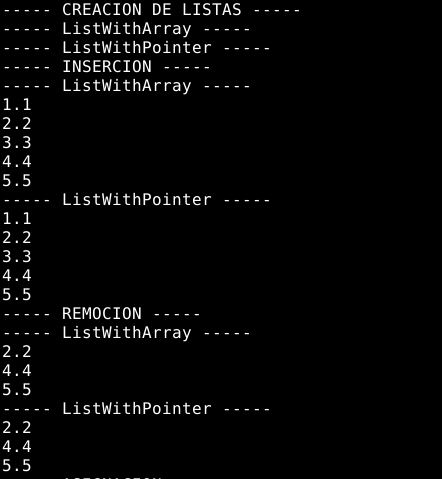
\includegraphics[width=0.4\textwidth]{img/salida01.JPG}
\caption{Salida del programa parte I}
\label{fig:Figura1}
\end{figure}

\begin{figure}[H]
\centering
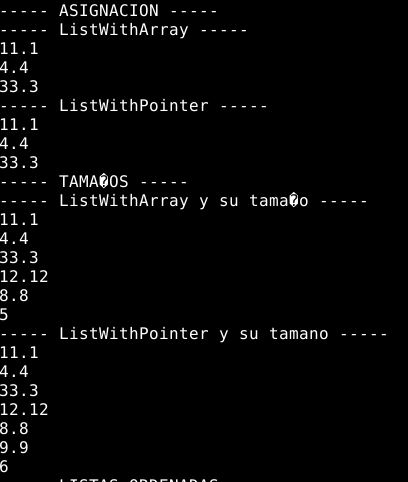
\includegraphics[width=0.4\textwidth]{img/salida02.JPG}
\caption{Salida del programa parte II}
\label{fig:Figura2}
\end{figure}

\begin{figure}[H]
\centering
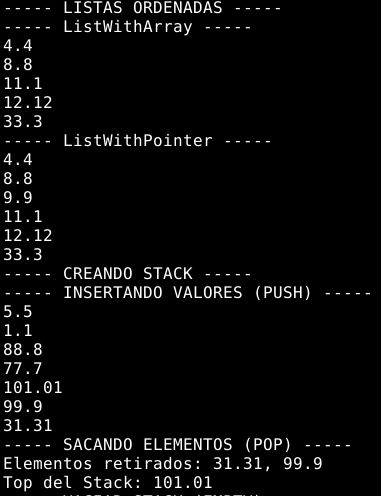
\includegraphics[width=0.4\textwidth]{img/salida03.JPG}
\caption{Salida del programa parte III}
\label{fig:Figura3}
\end{figure}

\begin{figure}[H]
\centering
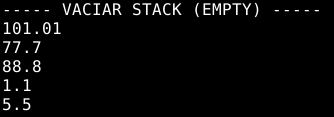
\includegraphics[width=0.4\textwidth]{img/salida04.JPG}
\caption{Salida del programa parte IV}
\label{fig:Figura4}
\end{figure}
\newpage
\nocite{*}
\bibliographystyle{plain}
\bibliography{biblist.bib}

\end{document}